\documentclass{article}

% if you need to pass options to natbib, use, e.g.:
% \PassOptionsToPackage{numbers, compress}{natbib}
% before loading nips_2016
%
% to avoid loading the natbib package, add option nonatbib:
% \usepackage[nonatbib]{nips_2016}

\PassOptionsToPackage{numbers,sort&compress}{natbib}
\usepackage[final]{nips_2016} % produce camera-ready copy

\usepackage[utf8]{inputenc} % allow utf-8 input
\usepackage[T1]{fontenc}    % use 8-bit T1 fonts
\usepackage{hyperref}       % hyperlinks
\usepackage{url}            % simple URL typesetting
\usepackage{booktabs}       % professional-quality tables
\usepackage{amsfonts}       % blackboard math symbols
\usepackage{nicefrac}       % compact symbols for 1/2, etc.
\usepackage{microtype}      % microtypography
\usepackage{graphicx}
% \usepackage{float}

\title{Spotify Analysis}

% The \author macro works with any number of authors. There are two
% commands used to separate the names and addresses of multiple
% authors: \And and \AND.
%
% Using \And between authors leaves it to LaTeX to determine where to
% break the lines. Using \AND forces a line break at that point. So,
% if LaTeX puts 3 of 4 authors names on the first line, and the last
% on the second line, try using \AND instead of \And before the third
% author name.

\author{
  s2554720\\
  %% examples of more authors
  \And
  s2584336\\
 \And
  s2612761\\
}
\begin{document}
\maketitle
\begin{abstract}
This study focuses on the analysis of Spotify’s “Top 200” playlist and the development of predictive models on the song attributes to determine if a song would become a hit and remain in the top rank 70 in time based on a dataset from 2017 to 2023. Four supervised learning algorithms were tested: Logistic Regression, Random Forest, Naive Bayes, and Neural Networks. The Random Forest model achieved the highest predictive F1-score at 0.823, while the Naive Bayes model reached 0.615 as its F1-score. Both significantly outperformed Neural Network and Logistic Regression at 0.38 and 0.120 F1-score respectively. Further unsupervised learning via K-means clustering identified 5 distinct groups of songs based on song features. This clustering allows new songs to be categorized with similar existing hit songs. The results demonstrate the feasibility of applying machine learning techniques to predict musical success and understand similarities between hit songs. This hit prediction system could assist music producers and companies in planning promotional strategies.
\end{abstract}

\section{Introduction}
Digital music streaming platforms like Spotify have drastically changed the music industry. These platforms have successfully responded to the challenges brought by recent digital disruptions in the media and music industries. This revolutionary impact of digital streaming culture is significantly associated with tech giants such as Prime Music, YouTube, and Apple Music, showing a significant influence on our collective musical future \cite{fleischer2017discovering}. In this regard, Spotify, as one of the world's largest music streaming platforms, is at the vanguard of this cultural shift, profoundly transforming how people discover and engage with music \cite{pinter2020p4kxspotify} \cite{jones2022competing}.

Spotify enables users to access huge music collections in a variety of contexts and genres. In this regard, navigating these huge music collections and finding music that suits one's interests could be challenging. Therefore, investigating playlists to get a better understanding of song characteristics holds the possibility of more tailored and improved music recommendations, which will improve the overall music-listening experience.

Spotify's huge song database with its metadata has been used in various studies to examine the factors affecting a song's popularity. These studies have used machine learning techniques for top song predictions, customer enteric experience and many more. Gulmatico et al. used music metrics to predict a song's popularity. Their findings indicated that the random forest classifier achieved the highest accuracy rate of 89\%; this makes it suitable for future song popularity predictions\cite{gulmatico2022spotipred}. To improve model selection, Kirasich et. al. \cite{kirasich2018random} evaluated the classification performance between random forest and logistic regression for datasets with various underlying structures. In this regard, to simulate classifier models and performance metrics, a model evaluation tool was developed, indicating that logistic regression has higher accuracy when variance in explanatory and noise variables increases. However, the random forest had higher true positive rates and false positive rates for datasets with increasing noise variables. 
Khan et al. \cite{khan2022effect} presented a model to predict a song's popularity on Spotify. The model used a database consisting of songs that have already appeared in the Top 50 Global ranking and those that have not. Using the database, the model extracted information about songs, including their dancing, acoustic, and instrumental characteristics. In a study \cite{al2020cluster}, a cluster analysis was performed on the Top 100 Trending Spotify Songs of 2017, with 10 attributes, including danceability, energy, loudness, speechiness, acousticness, instrumentalness, liveness, valence, tempo, and duration. The findings indicated that low instrumentality and high danceability led to the song's popularity.

Music popularity prediction and song recommendations are two key applications of machine learning in the music streaming domain. The main goal of this study is to leverage machine learning models for both predicting the popularity of songs based on provided attributes as well as clustering songs by common characteristics. Machine learning approaches were examined to predict whether a song will be popular in time using song attributes of Spotify's Top 200 playlists from 2017 to 2023. Factors associated with the song's popularity regardless of the artist are identified and are used to build these models. Additionally, an unsupervised k-means clustering algorithm groups the playlist dataset into clusters of songs with similar features.

\section{Exploratory data analysis}
EDA is understanding the distributions, getting an idea of the kind of values and their range, and understanding the nature of data before further analysis\cite{ghosh2023understanding}. The dataset encompasses lists of the top 200 songs published from January 2017 to May 2023. It comprises 9,161 unique song titles and 2,928 artists. Song attributes, such as danceability, energy, loudness, speechiness, acousticness, instrumentalness, and valence, are numerical and continuous in nature, offering insights into the composition of the songs. The density distribution of these attributes of unique songs is shown in Figure 1. Valence followed a near-normal distribution with a mean of around 0.5. Speechiness and acousticness were right skewed, with most songs falling in the range of 0.1 but a long right tail out to over 0.4 and 0.8 respectively. Danceability followed a slightly left-skewed bell curve distribution. Overall these density distribution plots have enabled exploratory data analysis regarding the underlying spread and characteristics of key song attributes.

\begin{center}
    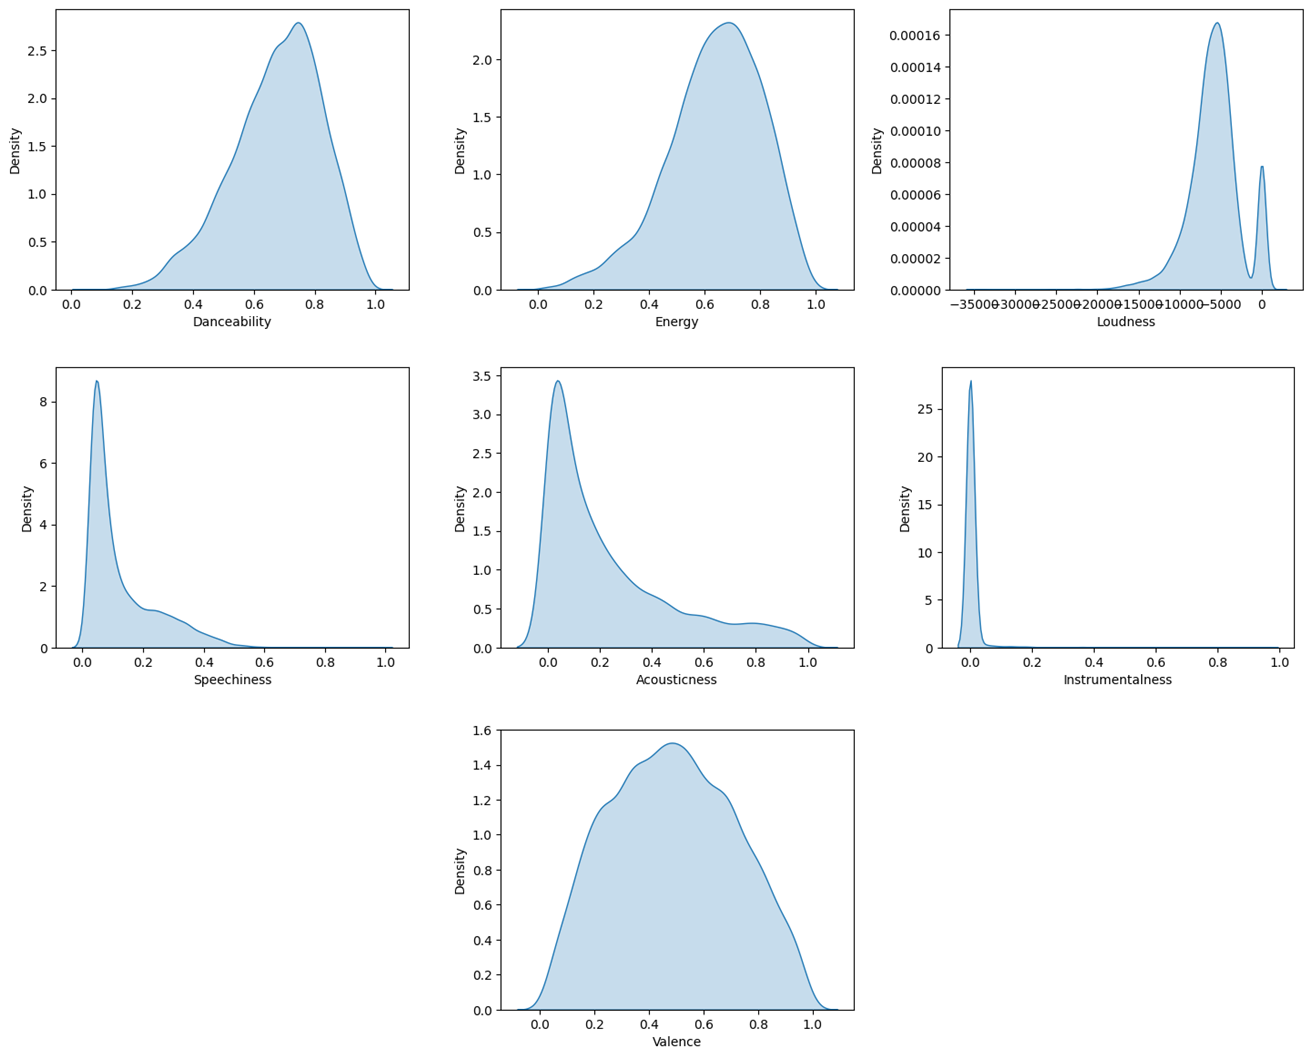
\includegraphics[width=0.7\textwidth]{kdefinal.png}
\end{center}
\begin{center}
    \footnotesize{Figure 1- Kernel Density distribution of song attributes in Spotify dataset}   
\end{center}

The correlation matrix which quantifies the association between the song attributes, rank and points of the given dataset, shows that rank and points have a strong positive correlation while other song features are not co-related to each other or ranks. As nothing about the song changes (even the artist remains the same), the factor that influences the rank is missing. Hence, how a song comes up in the rank list cannot be predicted by considering the linear relationship of ranks and song features. To further analyze what impacts rank, we look at correlations between rank and time since a song's release. This checks if there are patterns in how a song's ranking changes in the time following its release. Songs that gradually move up the rankings over time would show a negative correlation, indicating they gain popularity long after release. Songs that quickly achieve a high rank after release but then sharply drop off would show a strong positive correlation. Analyzing the correlation with time allows us to filter songs based on patterns in their ranking trajectory, rather than just their current rank. Songs with a consistent upward trajectory may be more popular songs than the songs that spike early but then quickly fade. This time-based correlation analysis provides additional insights into what drives ongoing popularity.

To focus on these high-quality songs that gained popularity in time, we considered songs that had an average rank of 70 or less during the time they were on the list. Our goal is to create a feature indicating whether a song is a "hit" based on the ranking criteria that have an average rank of 70 or less and a lower correlation. If the rank was decreasing over time (e.g. 3, 2, 1), the correlation with respect to time would be more negative and songs would more likely be classified as hits. If rank increased over time, the correlation would be positive and fewer songs would be classified as hits. To create the "hit feature", we assigned a value of 1 to songs that met our quality criteria average rank $\leq$ 70 and correlation less than 0.1. All other songs were assigned a 0 value for the "hit feature".
Figure 2 \& 3 shows the trend of the song "Peso Pluma: Por las Noches" which comes on the list at a lower rank but in due time reaches the top of the list. Whereas the song "Lewis Capaldi: Someone You Loved " hits the list at a top rank and goes down in due time. Looking at these trends the question arises which songs perform best in time and go from bottom to top and gain popularity based on the song's features? This forms the basis of the predictive task taken up in this study.

\begin{center}
  \centering
  \begin{minipage}{0.45\textwidth}
    \centering
    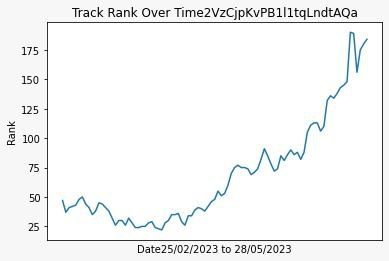
\includegraphics[width=\linewidth]{1.jpg}
    \footnotesize{Figure 2 - Rank vs date for Peso Pluma: Por las Noches}
  \end{minipage}\hfill
  \begin{minipage}{0.45\textwidth}
    \centering
    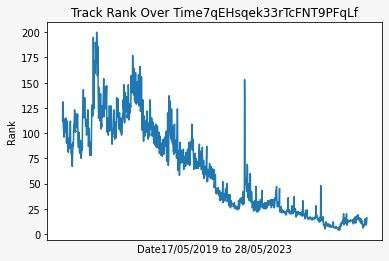
\includegraphics[width=\linewidth]{2.jpg}
    \footnotesize{Figure 3 - Rank vs date for Lewis Capaldi: Someone You Loved}
  \end{minipage}
\end{center}

After removing irrelevant attributes like artist name and nationality, our dataset contained 651,936 songs with 8 remaining attributes. Based on our hit criteria, 12\% of songs (78,232) were labeled as hits with a 1 value, while the remaining 88\% (573,704) were non-hits with a 0 value. Since the number of hits and non-hit songs was imbalanced, we used the "resample" function from scikit-learn to resample the dataset to achieve class balance. The re-sampled dataset contains 1,161,184 songs, with equal numbers of hits and non-hits. We split the resampled data 80/20 into training and test sets. The training set will be used to build models to predict song hits, while the test set will evaluate model performance on new unseen data.

\section{Learning methods}
There are various machine learning-based classification algorithms that take input as numerical values to make binary classification task (class 1 indicates the song exhibit characteristics of being a hit and the opposite for class 0 ). As we are aware of the target values supervised learning models can be used. A few of the supervised machine learning models are implemented in this study namely Logistic Regression, Naive Bayes, and Random Forest, and in addition to that Neural network-based approach is also discussed and implemented.

Logistic regression could be an appropriate model for predicting song popularity as it models the probability of a song being a hit based on multiple features. The utilization of the sigmoid activation function so that the class probability lies between 0 and 1. It works on the assumption that there is a linear relationship between the log odds of a song being a hit (the target value - $y$ ) and the numerical features we have on audio characteristics $(x_{1},.....x_{6})$.  While this linearity assumption may not fully hold for complex music data, logistic regression has some benefits in terms of interpretability and avoiding overfitting as long as the features demonstrate at least some association with the outcome. Because we have a relatively straightforward binary prediction target, the computations are fast and the model itself can be fit with at most a moderate number of audio features as predictors. It can provide interpretability with its coefficient values\cite{Schielzeth2010SimpleMT}.

In the context of Naive Bayes, the assumption made is that the audio features are conditionally independent of the others given the value of the response variable. Naive Bayes can provide useful predictions efficiently as long as some associations exist between individual features and the outcome. Given the associations, the Bayes theorem can be applied to calculate the probability of a hit song based on the combination of numerical audio features. Despite its strong feature independence assumption, Naive Bayes can often perform surprisingly well in many contexts\cite{Zhang2004TheOO}. 

Random forest has widespread use and is effective for prediction problems involving both categorical and continuous variables. The random forest ensemble method also reduces overfitting compared to single decision trees \cite{Dedja2022ExplainingRF}, further the flexibility to capture complex features is a key advantage. Its ability to model complex interactions among the song features without overfitting quickly by making use of ensemble decision tree learning increases the model to perform more robustly. Random Forest is implemented by training each tree on a subset of features and building an ensemble, the algorithm can capture nonlinear relationships and higher-order interactions among song/acoustic features that influence the target value.

Finally, neural networks were included given their power in modeling complex nonlinear relationships when provided with sufficient training data. The multilayer perceptron architecture is well-suited for tabular data like this dataset. With their universal function approximation capabilities, neural networks have achieved state-of-the-art results across various domains\cite{Hajela1992NeuralNI}\cite{Iannella2001ASN}.  The model transforms input audio features through multiple nonlinear layers and can capture complex relationships between song properties with respect to the result.

The performance of these diverse algorithms was compared to determine the most suitable approach for predicting potential hit songs using the set of audio, release, and artist features available. The performance of these algorithms was compared to determine the optimal approach for predicting potential hit songs using the available features.

Logistic Regression is implemented for the dataset with the following set of hyperparameters - solver - newton-cholesky as n\_samples >> n\_features and l2 penalty is being used. The Naive Bayes is being implemented using the standard hyperparameters. In Random Forest the max\_depth of the tree is assigned to be 5, this way overfitting the data can be prevented to an extent. For the Neural Network, the implemented model consists of architecture and hyperparameters as follows,  one input layer with 64 neurons, 3 hidden layers with 32, 16, and 4 neurons respectively, the ReLU activation function was used for the hidden layer and the sigmoid function used for output layer, Adam optimizer is used and 'binary\_crossentropy' loss is being taken into consideration(as the classification is binary). The model is trained for 50 epochs. Further to avoid overfitting callbacks are initialized which implement Earlystopping and reduce\_learning\_rate based on the validation loss.

In addition to the supervised models, k-means clustering as an unsupervised learning model was applied to the Spotify dataset to effectively group the available songs into distinguishable unique groups based on the song/acoustic properties. K-means clustering aims to divide observations into k clusters where each observation belongs to the cluster with the nearest mean. This unsupervised technique was selected to identify groups of songs that have similar audio features\cite{Wlfing2012UnsupervisedLO}, under the hypothesis that songs within the same cluster may share common traits that contribute to their success or appeal. K-means is an efficient clustering method for large datasets like this song data. The goal was to gain additional insight into key audio factors that may distinguish hits from non-hits. The clustering was performed by varying k to determine the optimal number of clusters for this data.

To determine the number of clusters the elbow graph is plotted and it's observed that the 5 K-means clusters are sufficient for the given dataset.

 
\section{Metrics}
In evaluating our binary classification model for predicting whether a song is popular or not, we employed a comprehensive set of metrics to assess its performance. While accuracy is a common metric, it may not be the most suitable choice, especially in situations with given imbalanced dataset where the number of popular songs might be significantly lower than non-popular ones. Instead, we prioritized metrics like F1-score, ROC-AUC, precision, and recall. The F1 score considers the balance between precision and recall, providing a holistic measure of a model's performance within the hit and non-hit classes. ROC-AUC, on the other hand, captures the trade-off between true positive and false positive rates at different thresholds, offering insights into the classifier's overall discriminatory power. Precision and recall complement these metrics by focusing on the model's ability to correctly identify hit songs and minimize false positives. Given the potential class imbalance in predicting popular songs, these metrics, particularly F1-score and ROC-AUC, offer a more nuanced and informative evaluation of our model's effectiveness.

\section{Results}
All the classification models after fitting to the training dataset were tested on the test data. The performance of the models with the evaluation matrix as described is tabulated in Table 1. The random forest model achieved the highest F1-score at 0.823, significantly outperforming Naive Bayes which had an F1-score of 0.615, and logistic regression which had an F1-score of 0.120. Despite the good accuracy, neural network had a F1-score of 0.38. Overall, the random forest model demonstrated the most balanced performance, with strong precision in predicting hits combined with reasonably high recall for hits. The relationship between the input features and the target is complex and nonlinear as discussed in the EDA section. Logistic regression assumes a linear relationship hence it failed to capture the true relationship between audio characteristics and popularity, and it does not explicitly model interactions between features., while Naive Bayes relies on strong feature independence assumptions which are not necessarily followed by the given dataset hence the low accuracy. In contrast, random forests and neural networks can model complex nonlinear relationships and interactions between variables, but neural networks lack transparency in the model as the model has high training accuracy but low F1 score indicating overfitting due to lack of enough variations in the dataset. 

\begin{center}
\centering
  \begin{tabular}{|c|c|c|c|} \hline
    Model& F1 score & Recall & Precision \\ \hline
    Random Forest& 0.823& 0.92& 0.73\\
    Neural Networks& 0.38& 0.49& 0.5\\
    Naive Bayes& 0.615& 0.75& 0.51\\
    Logistic Regression & 0.120& 0.07& 0.55\\ \hline
  \end{tabular}
\end{center}
\begin{center}
    \footnotesize{Table 1- Performance Matrix of models}
\end{center}

The random forest model achieved the highest AUC of 0.79. Its ROC curve shows strong classification ability, with the TPR consistently above 0.6 while the FPR remains below 0.2 over most threshold values. This indicates the random forest can achieve high true hit detection rates with low false alarm rates for non-hits. The neural network with an AUC of 0.49 suggests that the neural network is nearly performing as a random generator. This suggests that less than half of the time, the model ranks a random positive case higher than a random negative one. Similar patterns of AUC for ROC are being displayed by logistic regression and naive Bayes as well. It can be inferred that despite models that have high accuracy the performance of certain models might be closer to random guessing, and using ROC we are able to rightfully conclude that amongst the considered models random forest is performing the best.

Feature importance scores were extracted from the random forest to gain insight into which song attributes were most influential in predictions as seen in figure 5. The 3 most important features according to the model were: Energy, danceability and speechiness. Danceability and energy were the top drivers of hit classification, aligning with the hypothesis that songs with more upbeat, danceable rhythms tend to become popular hits. Speechiness also had an outsized impact, with increased speechiness correlated to hits. More acoustic tracks, characterized by minimal electronic instrumentation, were predictive of non-hits. Songs with higher instrumentalness were less likely to be big hits based on the model. Intuitively, heavily produced pop songs tend to gain more mainstream success than simpler instrumental artists. While not among the very top features, acousticness also has moderately high importance.

\begin{center}
  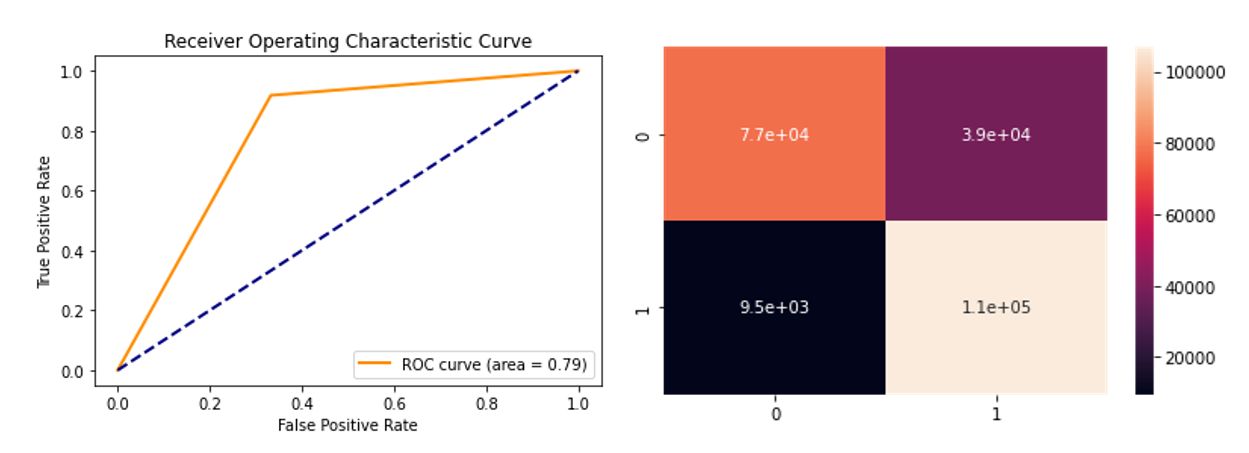
\includegraphics[width=1\textwidth]{ROC for random forest.png}
\end{center}
\begin{center}
    \footnotesize{Figure 4 - ROC and confusion matrix for random forest} 
\end{center}



\begin{center}
  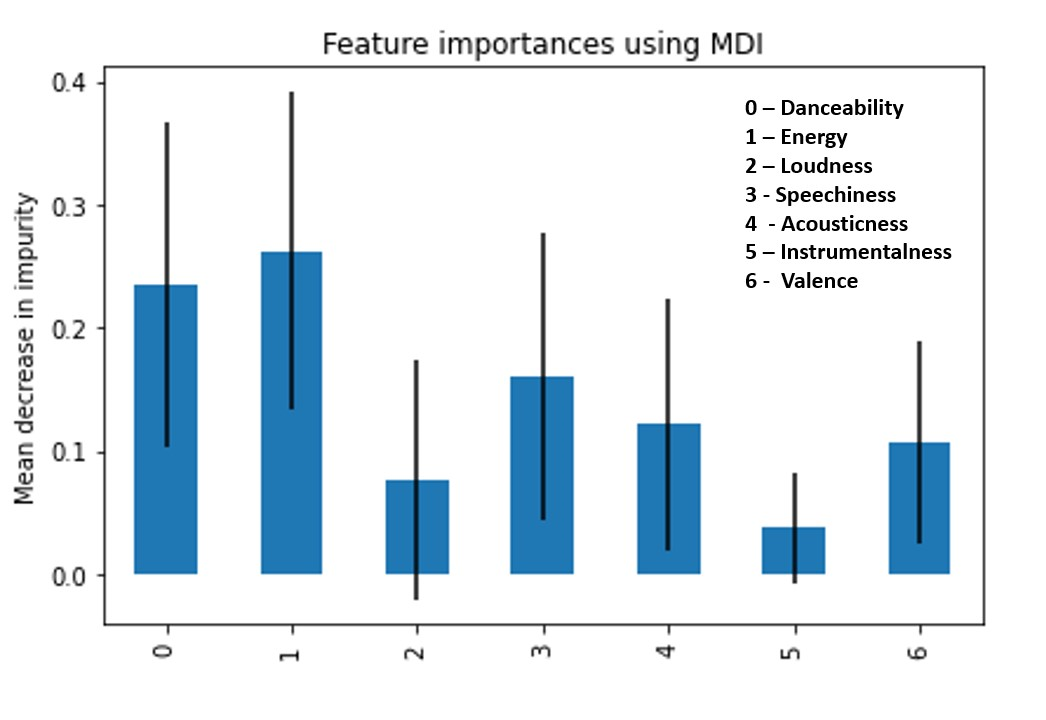
\includegraphics[width=0.6\textwidth]{output.png} % Replace 'example-image' with the filename of your actual image
\end{center}
\begin{center}
  \footnotesize{Figure 5 - Features for random forest}
\end{center}

For K-means clustering the optimal number of clusters was determined to be k=5 using the Elbow method on the within-cluster sum of squared errors plot. This yielded 5 distinct clusters varying in size from 298 to 3329 unique songs each. The size and number of songs that are hit are summarized in Table 2. These clusters reveal associations between certain audio factors and hit potential. In particular, cluster 2 and 3 was most correlated with hit songs, while cluster 4 had fewer hits. 

\begin{center}
\centering
  \begin{tabular}{|l|c|c|c|c|c|}
    \hline
    Clusters & Cluster 1 & Cluster 2 & Cluster 3 & Cluster 4 & Cluster 5 \\
    \hline
    Size of Cluster & 1456 & 3078 & 3329 & 298 & 1000 \\
    \hline
    Number of hit songs in the cluster & 43 & 117 & 112 & 8 & 29 \\
     \hline
 Percentage of hit songs& 2.95& 3.80& 3.36& 2.68&2.90\\\hline
  \end{tabular}
\end{center}
\begin{center}
    \footnotesize{Table 2 - Distribution of songs within the clusters}
\end{center}

\section{Conclusions}
Random forest works the best among the classification models with respect to their corresponding F1 scores. The random forest model and K-means clustering model can be used for the prediction of the song's hit using song attributes.  Provided a new song, companies and artists can use these two models to know whether the new song will be a hit or not, and under what cluster that new song falls into. Segmenting songs into behaviorally distinct groups could help guide marketing and recommendations based on audio similarity rather than relying solely on genre labels.


\pagebreak
\bibliography{refs.bib}
\bibliographystyle{plain}

\appendix


\section{Contribution}
s2554720 - project ideation, EDA, report writing, result analysis

s2584336 - project ideation, EDA, report writing, model implementation

s2612761 - project ideation, EDA, report writing, literature review
\section{GenAI}
Generative AI was used to write basic codes for plotting the figures, grammar correction and \LaTeX code for figure adjustment.

\section{Additional Information}
This is the first appendix section.
It is known that some songs become popular due to the presence of a particular singer, but because of their qualities, they might lose their top ranking. Here we concentrate on accessing songs that show song qualities based on which they hit the chart. Hence, we consider only song features to analyze a song's ranking. If a date song reaches the top 200 and comes up from bottom to top, then it has performed well, irrespective of the artist. This is entirely dependent on the attributes of the song that make it trendy. To find these types of songs, we try to find the correlation of a song’s rank with respect to dates and use this correlation to find the performance of the song. As a result, the lower the correlation, the better the performance of the song. (If the initial song rank is 50, gradually the song rank gets increased to 30, 20, 10, and so on.) (The correlation of ranks w.r.t date will be negative.)

Below figure represents the top 10 artists with the highest count of unique songs within the top 200 list. This data enables us to gain valuable insights into the artistic preferences and styles of these musicians. It also equips us with the ability to make informed predictions regarding the potential popularity of future songs within the repertoire of these artists.
To determine which nation produces the most top-ranking songs, we have generated a graph showing the number of unique song titles for artists from each respective nation. As depicted in Figure 2, it becomes evident that the United States is the nation with the greatest number of top-ranking songs.
\begin{center}
  \centering
  \begin{minipage}{0.5\textwidth}
    \centering
    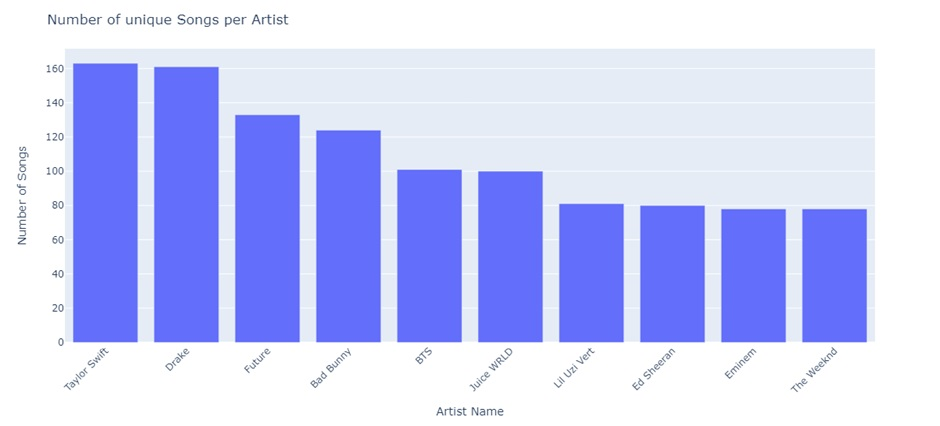
\includegraphics[width=\linewidth]{Untitled1.jpg}
    \footnotesize{Number of unique songs per artist.}
  \end{minipage}\hfill
  \begin{minipage}{0.5\textwidth}
    \centering
    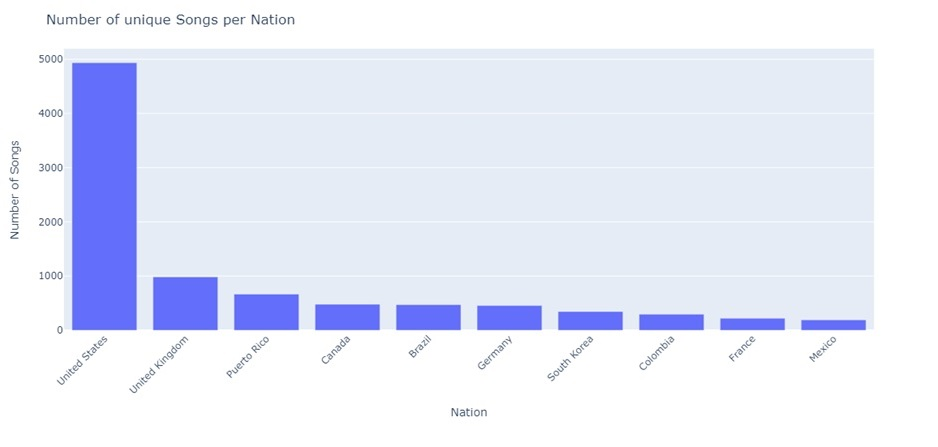
\includegraphics[width=\linewidth]{Untitled2.jpg}
    \footnotesize{Number of unique songs per nation.}
  \end{minipage}
\end{center}
\section{K-means elbow graph, K means graph centers}
The elbow method is used technique to determine the optimal number of clusters K in K-means clustering as shown in the figure. The idea is to run K-means clustering on the data for a range of values of K (here from 1 to 35). Sum of Squared Error within clusters is calculated for each value of K and plotted on the y-axis with the number of clusters on the x-axis. This curve looks like an arm, with the "elbow" starting at k = 5 (meaning 5 is the optimal cluster indicating the best tradeoff.
\begin{center}
  \centering
  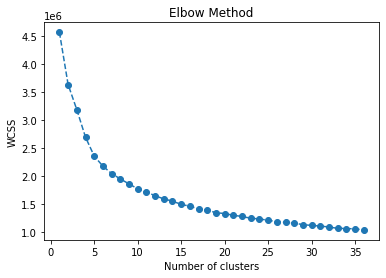
\includegraphics[width=0.6\textwidth]{k means elbowpng.png} % Replace 'example-image' with the filename of your actual image
\end{center}
\begin{center}
  \footnotesize{K means elbow method}
\end{center}

\section{Model accuracy of NN}

\begin{center}
  \centering
  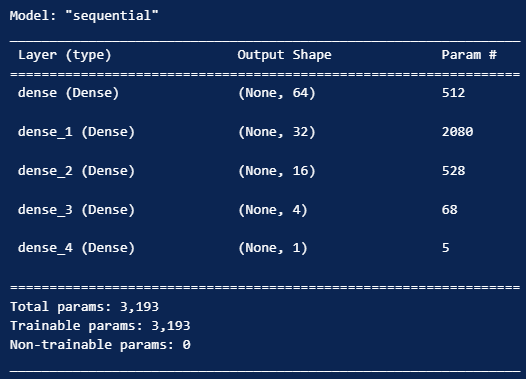
\includegraphics[width=0.6\textwidth]{NN model summary.png} % Replace 'example-image' with the filename of your actual image
\end{center}
\begin{center}
  \footnotesize{NN model architecture}
\end{center}
\begin{center}
  \centering
  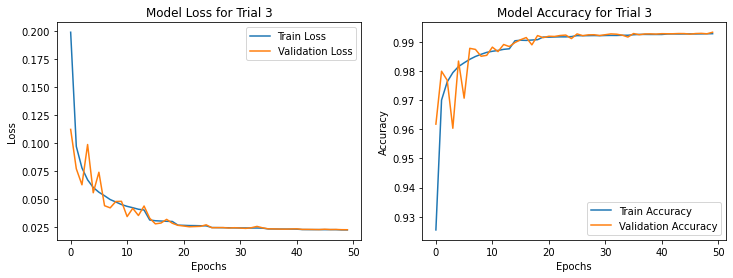
\includegraphics[width=1\textwidth]{NN model verbose.png} % Replace 'example-image' with the filename of your actual image
\end{center}
\begin{center}
  \footnotesize{Neural network model training and validation performance}
\end{center}



\section{Additional EDA-PCA}
Principal component analysis (PCA) was explored as a dimensionality reduction technique for the 7 song features.  An "elbow method" was utilized to determine the optimal number of components - where adding more components leads to marginal gains in variance explained. However, the plot below showing the variance explained per principal component did not reveal an obvious elbow point. The variance was fairly evenly distributed across many components, without a clear cutoff for dominant components. This indicates there may not be enough latent structure related to a few strong patterns in this data. Applying PCA then could lead to oversimplification and loss of signal.
\begin{center}
  \centering
  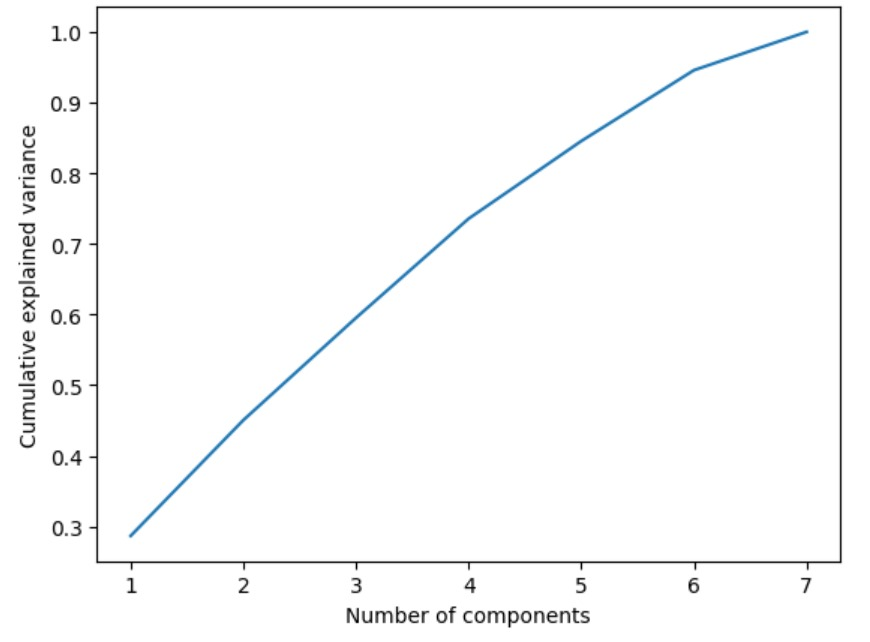
\includegraphics[width=0.6\textwidth]{PCA.jpeg} % Replace 'example-image' with the filename of your actual image
\end{center}
\begin{center}
  \footnotesize{Cumulative Explained Variance}
\end{center}
\end{document}

%%% Local Variables:
%%% mode: latex
%%% TeX-master: t
%%% End:
